\documentclass[journal]{vgtc}                % final (journal style)

\ifpdf%                                % if we use pdflatex
  \pdfoutput=1\relax                   % create PDFs from pdfLaTeX
  \pdfcompresslevel=9                  % PDF Compression
  \pdfoptionpdfminorversion=7          % create PDF 1.7
  \ExecuteOptions{pdftex}
  \usepackage{graphicx}                % allow us to embed graphics files
  \DeclareGraphicsExtensions{.pdf,.png,.jpg,.jpeg} % for pdflatex we expect .pdf, .png, or .jpg files
\else%                                 % else we use pure latex
  \ExecuteOptions{dvips}
  \usepackage{graphicx}                % allow us to embed graphics files
  \DeclareGraphicsExtensions{.eps}     % for pure latex we expect eps files
\fi%

%% it is recomended to use ``\autoref{sec:bla}'' instead of ``Fig.~\ref{sec:bla}''
\graphicspath{{figures/}{pictures/}{images/}{./}} % where to search for the images

\usepackage{microtype}                 % use micro-typography (slightly more compact, better to read)
\PassOptionsToPackage{warn}{textcomp}  % to address font issues with \textrightarrow
\usepackage{textcomp}                  % use better special symbols
\usepackage{mathptmx}                  % use matching math font
\usepackage{times}                     % we use Times as the main font
\renewcommand*\ttdefault{txtt}         % a nicer typewriter font
\usepackage{cite}                      % needed to automatically sort the references
\usepackage{tabu}                      % only used for the table example
\usepackage{booktabs}                  % only used for the table example

\onlineid{0}

\vgtccategory{Research}

\vgtcpapertype{system}

%% Paper title.
\title{Decision Support for Organizational Change (DSOC)}

\author{Rob Barwell and Eric Spero}
\authorfooter{
%% insert punctuation at end of each item
\item
 Rob Barwell and Eric Spero are with Carleton University. E-mail: robert.barwell/eric.spero@carleton.ca.
}

%other entries to be set up for journal
\shortauthortitle{Biv \MakeLowercase{\textit{et al.}}: Global Illumination for Fun and Profit}
%\shortauthortitle{Firstauthor \MakeLowercase{\textit{et al.}}: Paper Title}

\abstract{
DSOC is a novel way to visualize the complex problem of organizational change by allowing the user to quickly see where gaps exist in an organization, understand the gaps that exist, and help the user determine how they might fill the gaps.  This is supported by using email within an organization to model the flow from one employee to another.  This representation provide the most current and concrete representation of the organization and allows the user to make better decisions when faced with organizational change.
} 
\keywords{Organizational change, decision-making, information visualization}

%% ACM Computing Classification System (CCS). 
%% See <http://www.acm.org/class/1998/> for details.
%% The ``\CCScat'' command takes four arguments.

\CCScatlist{ % not used in journal version
 \CCScat{K.6.1}{Management of Computing and Information Systems}%
{Project and People Management}{Life Cycle};
 \CCScat{K.7.m}{The Computing Profession}{Miscellaneous}{Ethics}
}

%% Uncomment below to disable the manuscript note
\renewcommand{\manuscriptnotetxt}{}

%% Copyright space is enabled by default as required by guidelines.
%% It is disabled by the 'review' option or via the following command:
%\nocopyrightspace

\vgtcinsertpkg

%% Start document!

\begin{document}

\firstsection{Introduction}

\maketitle

The rise of the \lq gig economy\rq{}\cite{de2015rise,friedman2014workers} has forced society through a massive transition in the past two decades with people transitioning between jobs with greater frequency.  Historically, a person would obtain a job from high school or university and stay with a specific company until they retire.  This resulted in organizations that had minimal change, which could be easily managed. Modern organizations are forced to adapt with the shift to the gig economy and other non-traditional employment models.  

An organization is a social network\cite{scott1988social} of individuals engaged in complex \emph{interlocking contingencies}\cite{glenn2006complexity}: individuals in an organization are tightly interconnected, where the behaviour of one both depends on, and has subsequent consequences for the behaviour of others\cite{glenn2006complexity}. This feature of organizations means that the results of changes to its social structure (say, by adding or removing an individual) can be difficult to understand. Change is disruptive, and care must be taken to minimize any negative side-effects. The challenge of minimizing organizational disruption as a result of personnel change depends critically on understanding the effects of that change. In the gig economy, this challenge, and the need for tools that support it, is even greater. 

We aim to address this problem through \emph{information visualization}. Visualizations support thought by reducing the gap between the data, and the users' \emph{mental model} of the data\cite{yi2007toward}. A mental model is an internal representation of how something in the world works\cite{staggersmodel,norman2014some}. Wherever there is distance between the presentation of the data and our understanding of the data, mental work must be done so that understanding is possible. This type of mental work does not bring us closer to solving domain goals, but rather is a sort of unfortunate precursor for the really important work, and therefore should be avoided wherever possible\cite{paas2003cognitive}. Fortunately, the physical environment can be used to store information, which allows us to \lq off-load\rq{} mental work onto the environment\cite{wilson2002six}. Visualizations are essentially one way of effectively leveraging this property of the environment to aid thought.

\section{Background}

\subsection{Methodology}
The development of our visualization started with defining a methodology to help guide the design process.  We reviewed a number of papers in the area of evaluation of information visualization.  We found this area of research to be less concrete then other topics we had studied before.  The Challenge of Information Visualization Evaluation\cite{challengeofinfoviseval} paper we reviewed helped us to clarify our evaluation criteria and approach by validating our desire to present our design and findings to various user groups throughout the design process.  The Empirical Studies in Information Visualization: Seven Scenarios paper\cite{sevenscenarios} paper supported our desire to have an iterative approach similar agile software development.  The approach presented in the paper was Pre-design, design, prototype, deployment, and re-design.  This approach would also line up with using different user groups through the process.

Our design process involved us consulting three different user groups:
\begin{itemize}
	\item Group A - Government Department - This group represents users who address organizational change questions for a large Canadian Government department. 
	\item Group B - Academics - This group represents various academics at our University.
	\item Group C - Private Company - This group represents users at a private multi-national company who discovered our research during the design process.
\end{itemize}

Using these three groups we could gain informal feedback throughout the design process and strike a balance between modern visualization concepts that push the envelope and how a real world user would interpret those concepts.  By version 3 of our design we started to see the balance between the modern visualizations that the academics helped generate and the needs of real world users.  Our opinion is this approach should be standard in any visualization development to ensure there is a user adoption path that meets the needs of a broader audience.

After the initial design was explored we presented it to Group A who provided valuable feedback that contributed to the development of version 2.  Version 2 was then shown to Group B who helped define what version 3 would look like.  The academics were invaluable to help generate creative solutions to some of the challenges real users identified, but we were unable to solve on our own.  Version 3 was then shown to all Groups to validate the value they would obtain from our visualization.

\subsection{Problem Space}
Development of the design also led to reframing the original problem.  This required an iterative process to try and make sense of what we were looking for the visualization to help with.  This loosely followed a sense making model presented by Peter Pirolli and Stuart Card\cite{cognativetaskanalysis} where we started with a question eventually leading to a hypothesis and then through a validation process.  

The original problem was "How to address empty positions within an organization?"  This was a topic of interest to us as we know many organizations are facing organizational modeling problems within the current context of the "gig" economy where employees are constantly changing jobs and might only be with a company for a short term.  This leads to organizational charts that are quickly out of date and do not accurate reflect the true distribution and flow of work within an organization.  
Further discussion led to refining the problem as:
\begin{itemize}
\item “How do we support decision makers to minimize negative side-effects from organizational change?”
\item “How do we value a person in the organization?”
\item “How do we provide options to users to address vacancies within an organization?”
\end{itemize}
These statements can be further reshaped to what a user (i.e. managers) would understand the problem as.
\begin{itemize}
\item "Where is the gap?"
\item "How big is the gap?"
\item "What can I do about the gap?"
\end{itemize}

\subsection{Option Space}
Using a refined problem description we started to focus on how we would address these statements.  Using the work done by Ware on Visual Thinking Algorithms\cite[Chapter 11]{ware2012information} we decided to enumerate the steps a user would do manually to solve the problem statements and determine where visualization could help offload cognitive processes.

During our walk through with users we discovered they were sub dividing the problem and exploring it from different perspectives.  Some aspects of the process they found difficult was keeping track of what part of the problem space they had explored and modeling different views of the problem.  These tasks could easily be addressed with a visualization.  Below is a quick description of the different views that represent the users mental model of the probelm.
\begin{itemize}
\item Organizational - This places an employee in the traditional hierarchical organizational structure.  Commonly this is represented by a tree where the employee is a node and an edge is the link between nodes.
\item Process - This places an employee as part of a process where they receive information, process information, and output information to the next stage of the process.  Users typically used flow charts and other process diagrams to represent this view.
\item Redundancy - During the walk through we noticed it was most common to address the vacancy by re-distributing the workload within the group, however the users occasionally tried to find people that did similar tasks as replacement.
\end{itemize}

\subsection{Data}
During the exploration of the problem space we needed to identify what data we were going to present to the user with the visualization.  Building upon previous work from our colleague on information flow within an organization we decided to use emails.  We found the majority of communication within a modern organization is through email or instant messaging.  Using emails we would have an accurate and up to date model of how information flows through an organization.  

This concept resonated well with both the user and academic groups since it represented an improvement from the traditional organizational chart model which is typically out of date and does not capture the true contributions to the team of an individual employee.

The data model requires enrichment through the addition of value models.  One value model would be required to address the statement of "How big is the gap?" and the other value model would be required for "What can I do about the gap?".  Both value models presented below are rudimentary as the primary focus of this paper is the visualization problem and not the data problem.

\begin{itemize}
\item Gap Size - By modeling each employee as a node the emails between nodes would represent an edge with a weight of 1.
\item Gap Options - One option to address the gap could be redistributing the work to a "similar" employee. The value model we used to compare two employees is based on the overlap in the number of individuals they communicate with. 
\end{itemize}

\section{Design}

\subsection{Evolution of Design}
Our visualization was generated organically based on discussions with the groups identified in the previous section.  Based on their feedback adjustments were made to refine the design until the final design was reached.

Our design went through 3 major versions.
\begin{itemize}
	\item Version 1 - The initial design by the authors that focused on the organization and communication problem.
	\item Version 2 - Added the process and redundancy views.
	\item Version 3 - Refined the process and redundancy views to better align with the users mental model and how they interact with the visualization.
\end{itemize}

The most complex part of the design problem was creating a functional layout that conveyed the complex intricacies of organizational change.  The initial part of the design focused around understanding what tools we could leverage and how to fit them with the users mental model.  We required an intuitive layout that would allow the user to quickly understand the different views into the problem and allow the user to quickly understand where they are in their mental process.

\subsection{Layout}
\subsubsection{Structure}
The original design shown in Figure 1 had 3 viewing panes to try and convey the organizational perspective of information flow and the process perspective.  It attempted to do this using the standard organizational tree for organizational structure and a tree map to show the volume of communication between a selected individual and their communication links.  This view presented many challenges for users as they found it difficult to understand what the visualization was trying to communicate and weren't able to fit it into their mental model.  Based on feedback from Group A and reflection by the authors we determined that this concept was better communicated as a traditional supply demand problem as these were the words Group A typically used most often during the review of the first design.  This feedback allowed us to revise our design to a layout which was 2xN column representation that broke the problem in a supply / demand issue.  This allowed the users to better address the question of "How do we support decision makers to minimize negative side-effects from organizational change?" by understanding the impact and if required redistribute work based on available supply.

\begin{figure}
	\centering
	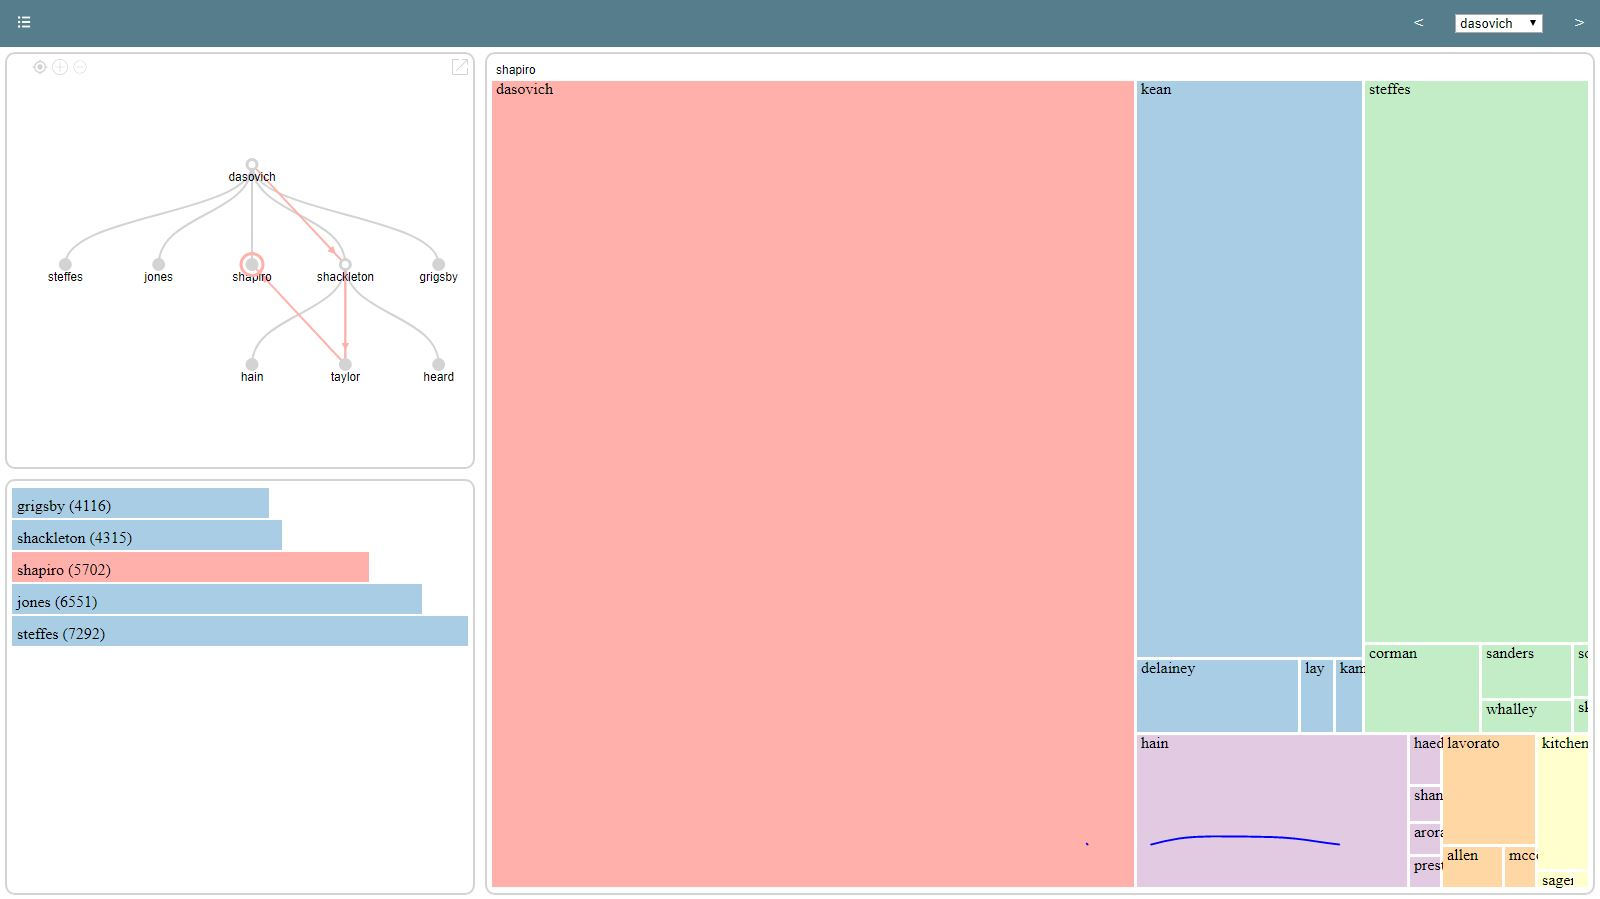
\includegraphics[width=\columnwidth]{pictures/version1.JPG}
	\caption{Version 1}
	\label{fig:global}
\end{figure}

The second designed shown in Figure 2 seemed to resonate better when shown to Group B and subsequently in version 3 for Groups A and C.  This allowed all groups to focus on the individual views within the visualizations versus focusing on the layout.

\begin{figure}
	\centering
	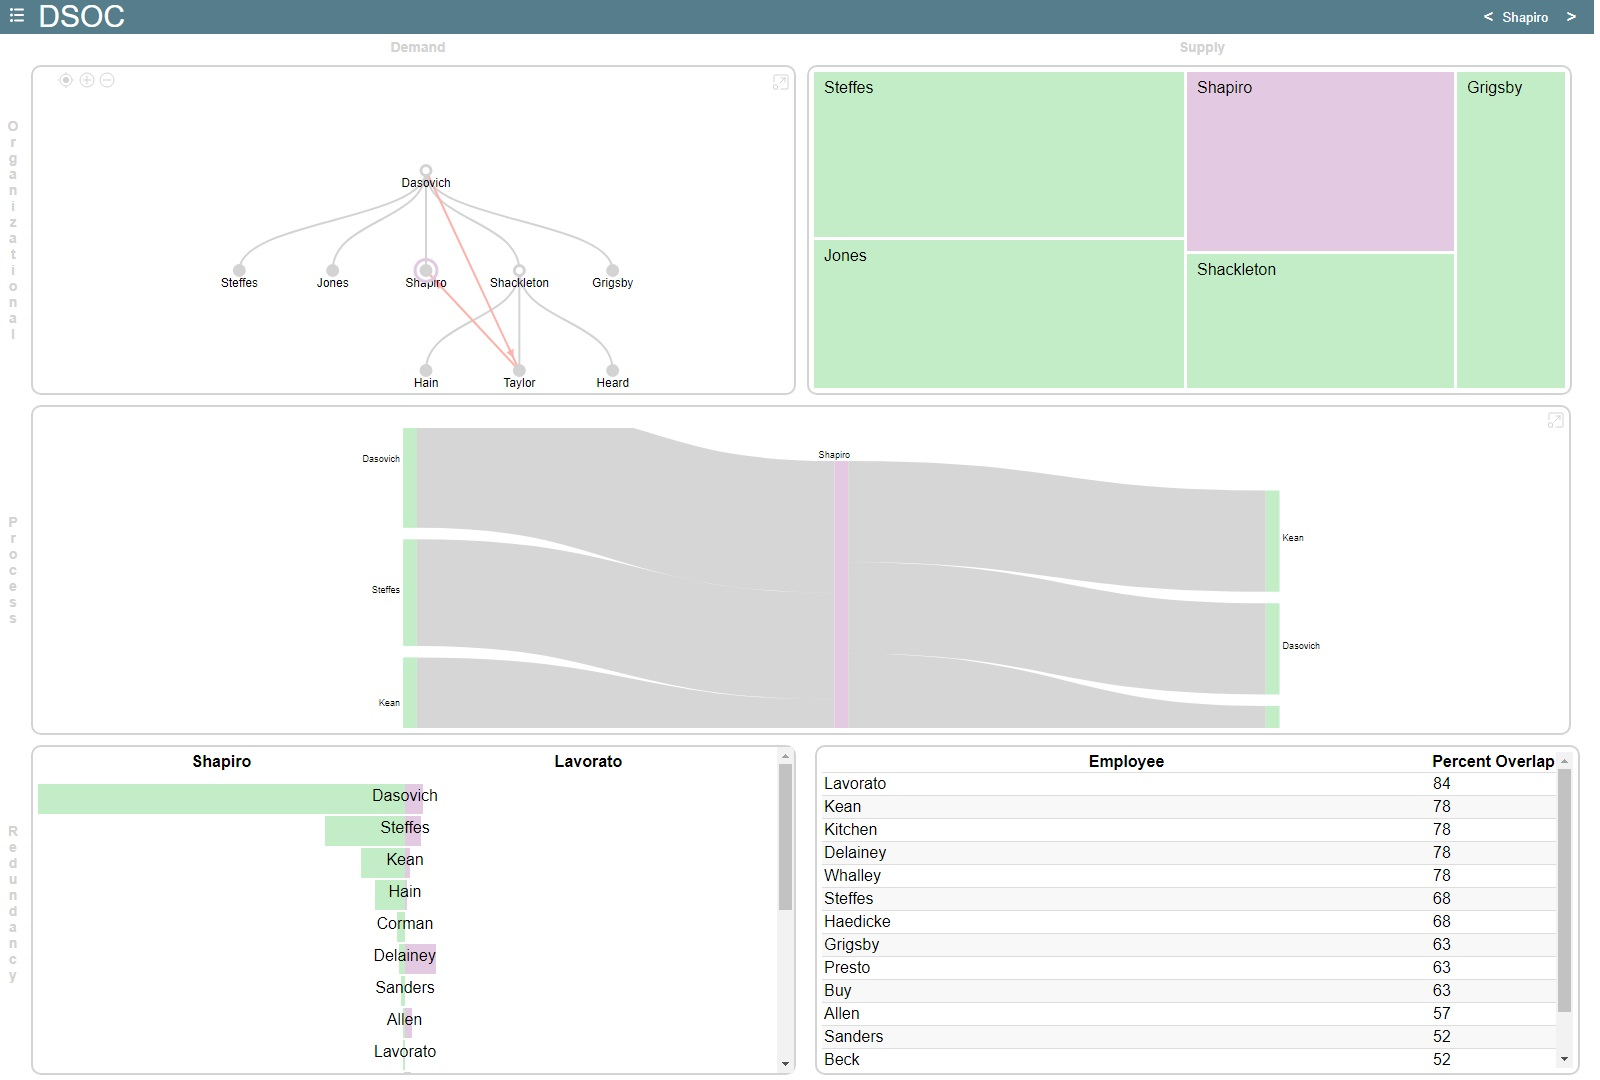
\includegraphics[width=\columnwidth]{pictures/version2.jpg}
	\caption{Version 2}
	\label{fig:global}
\end{figure}

Allowing each row to represent a different view of the problem space enables the flexibility to include different views in the future as more users trials of the system are conducted.

\subsubsection{Navigation}
Complimentary to the structure of the layout is how the user will navigate the layout.  Our goal was to provide the user with the freedom to explore the problem however they choose.  This required the support of a brushing scatter plot concept where the interactions within an individual sub view are reflected in the other sub views to ensure the user is always viewing the problem from a single data point through a number of lens.
As the user explored the problem it was also important to have a way for them to keep track of the problem space they have already explored.  This was a salient point that we found during the literature review with the quote “Information exploration is inherently a process with many steps, so keeping the history of actions and allowing users to retrace their steps is important”\cite{anafigueiras}.  This quote accurate describes how our users would interact with the system.  This was included by providing the user the option to display history as direction arrows or simply coloring the nodes in the organizational chart.  The user can then navigate the history using the navigation bar at the top of the screen.

\subsection{Organizational}
The organizational demand and supply view were the most consistent between version 1 and 3.  The demand view was modeled as a classical organizational tree structure as this paradigm was most aligned with the users current mental model of the problem.  During the design phase we uncovered a number of issues that we needed to address.
\begin{itemize}
	\item Actions - Some organizational trees can be large and we need to provide the user with the ability to zoom in and out of the tree, expand a node with children and select a node.  In version 1 we decided to use a single click to expand a node and select a node with one action and double click would zoom in and out of the tree.  Users in Group A found this confusing since opening the children of a node would also cause the node to be visited.  This was refined in version 2 where a single click selected a node, the double click would zoom in and out, and a right mouse click would open a node with children.  
	\item Highlight - During the initial design of version 1 we needed to come up with a creative solution to visualize the various states a node could have.  This includes: being selected, having children, being visited, and being filtered.  We originally experimented with glyphs and other icons, however this resulted in a visualization that was too "busy".  We settled on using concentric circles of different colors as shown in Figure 3 to denote various states of a node.  A node with children has a filled in circle.  A node that the user has visited appears in red.  A node that is filter is orange. And a node that is selected appears red.  We recognized the issue this might present for color blind people and also chose to vary the size of circle around the nodes to account for this.
	\item Navigation - Navigating large trees can present challenges for some users.  This was addressed by providing a real time filter where the user adjusts the filter parameters which are quickly reflected by circles appearing and disappearing around nodes in the tree that match the filter criteria.  Additionally the organization demand panel can be expand to fill the whole window to help the user navigate the entire tree.  Additional short cuts are provided at the top of the frame to center on the current selected node, expand all nodes, or collapse all nodes.
	\item Comparison - Version 1 of the design provide a feature that allowed the user to hover over a node and display the nodes they communicated with using a blue line.  This was further refined based on discussions with Group B to incorporate a weight.  This would then allow the user to see the overlap of where the employee is within the organization and which other employees they communicate with and how much.  This is denoted by the blue line in figure 3.
\end{itemize}

\begin{figure}
	\centering
	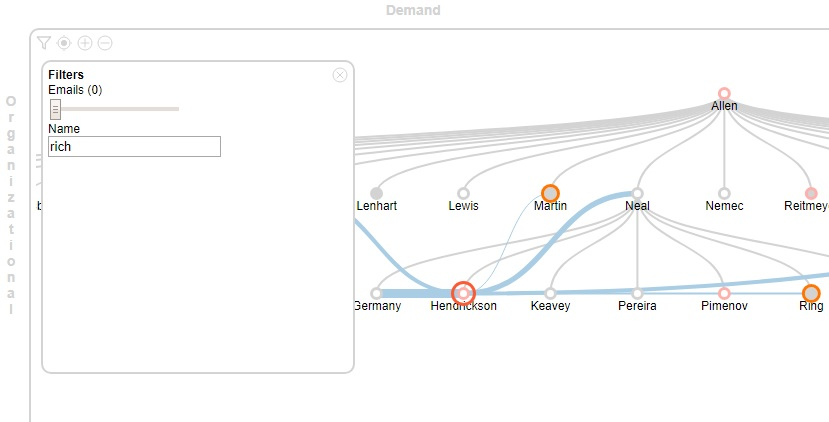
\includegraphics[width=\columnwidth]{pictures/orgdemand.jpg}
	\caption{Node Selection}
	\label{fig:global}
\end{figure}

The original organizational supply view was a horizontal bar chart as shown on the left side of figure 1.  In version 2 we experimented with changing this to a tree map as we wanted to show the relative size of each employee in a group compared to the others.  The space filling method\cite{shneiderman1992tree} as discussed in Ben Shneiderman original treemap paper was appealing since we did not know how large a group might be.  After discussion with Group B we decided treemaps were not appropriate since there were no levels to drill down to or group by.  It was also noted by Group A that a bar chart might be better for a comparison view point.  When the user clicks on any of the bars it will re-orient all views to select the employee.  The final vertical bar chart is shown in figure 4.

\begin{figure}
	\centering
	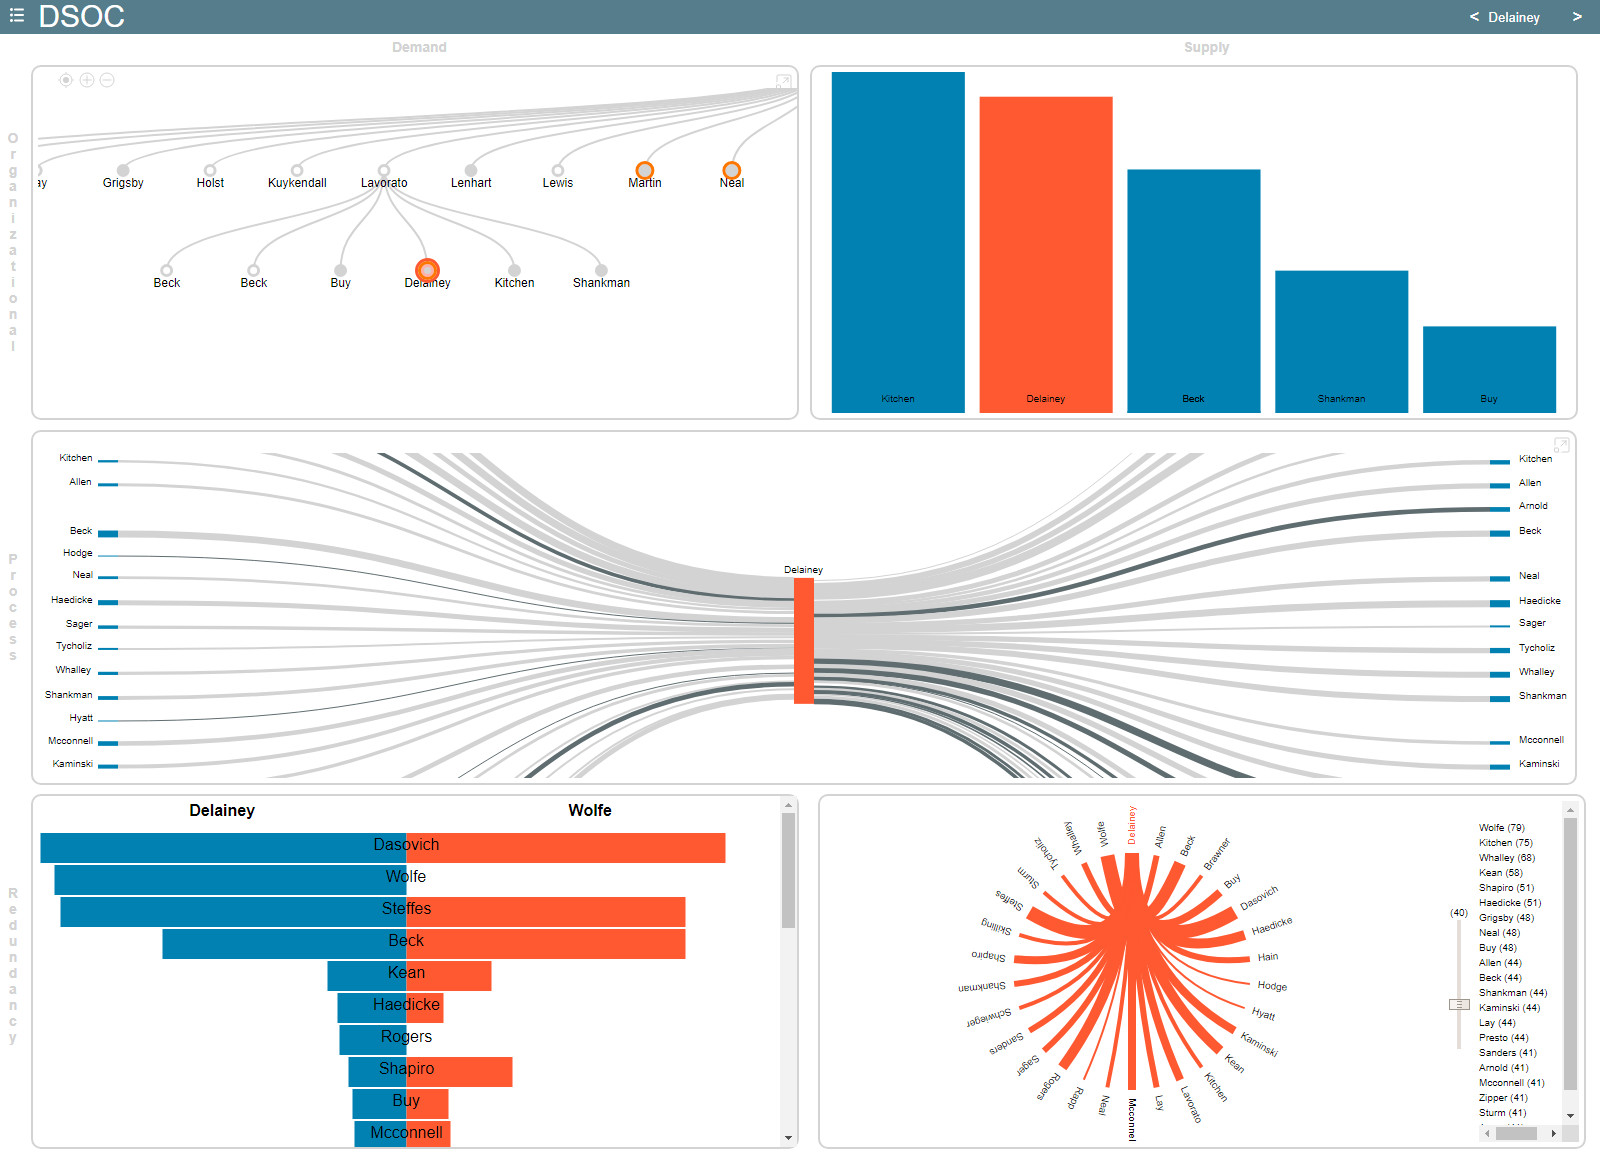
\includegraphics[width=\columnwidth]{pictures/version3.jpg}
	\caption{Version 3}
	\label{fig:global}
\end{figure}

\subsection{Process}

The process demand and supply view went through the most significant change between versions.  In version 1 a treemap was used to model the communication flow between the selected employee and those they communicate with.  This approach was great a showing the relative comparison of communication from the view of an employee, however Group A noted that this didn't really show flow of information and made it hard to determine what information started or ended with the selected employee.  Group A's suggestion was to investigate using a Sankey diagram.
In version 2 we added a Sankey diagram, however this version presented a number of challenges for Group B.  The unbalanced flow connections led the group to believe there was some sort of knowledge in the way it flowed from left to right which was simply a function of the layout algorithm and not used to communicate any information.  Additionally some communication links were large and made the visualization hard to interpret.  It was further compounded by users not being lined up on the left and right of the diagram.  Based on this feedback a complete redesign of the diagram was required.
Version 3 significantly changed the layout from version 2.  We scaled the links to make them easier to differentiate on the screen, color was added to denote links that either started or ended with the selected employee, and most significantly we lined up the communication flow so if a user was an incoming and outgoing communication flow they would appear at the same location on both the left and right hand side of the screen.
The unique nature of the Sankey diagram allows it to both show demand and supply.  This concept will be further discussed in the evaluation and discussion section.

\subsection{Redundancy}

The redundancy view was introduced in version 2 after discussions with Group A.  They thought it would be a "neat" idea to show similar people within an organization as a potential supply source to solve the identified gap.  Version 2 included a simple implementation where a back to back bar chart was used to help the user determine if the supply lined up with the demand and a table allowed the user to select the best supply based on the value model discussed in the previous section.
Group B had some challenges with the supply part of the design as a table wasn't how users typically compared two options.  This led us to investigate a number of options including hierarchical edge bundling and chord diagrams to try and show the overlap between two selections.  The chord diagram presented challenges since the selected employee would fill the entire circle making it hard to differentiate between the different paths.  The hierarchical edge bundling had the challenge of not showing the relative size of each connection.  This was over come by merging the two concepts to create the palm tree diagram.  This diagram allows the user to hover over the list of recommended users which was the table in version 2 and see the comparison.  This is shown in figure 5.  The slider also allows the user to adjust the cut off of the list in real time to try and narrow the scope of comparison without discounting employees that might have poor overlap with other employees.  This approach seemed to resonate well with all user groups in version 3 as it was flexible to an employee with many connections and provided instantaneous feedback to the user. 

\begin{figure}
	\centering
	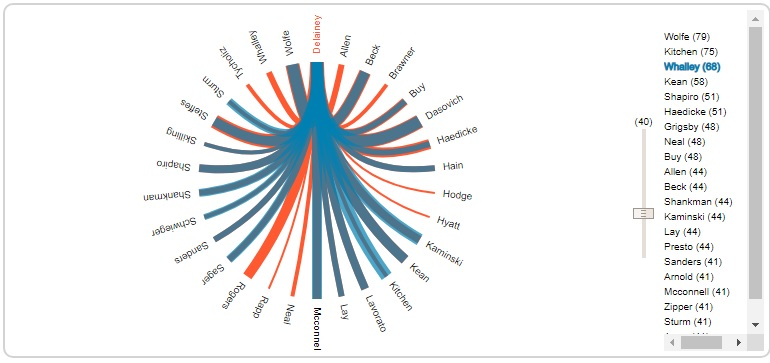
\includegraphics[width=\columnwidth]{pictures/palmtree.jpg}
	\caption{Palm Tree}
	\label{fig:global}
\end{figure}

\section{Implementation}
Each version of the design was implemented using MySQL, PHP, HTML, CSS, and Javascript using the D3 library.  A number of visualization systems were contemplated, however D3 was chosen due to its maturity level and flexibility to visualize our designs.

\subsection{Data}
Email (SMTP) header information was used to implement the value model discussed in the previous sections.  Alternative value models later in the paper.

To demonstrate our value model we chose the popular Enron email data set.  This data set was originally made public during the Federal Energy Regulatory Commission investigation.  It contains the emails of approximately 150 users in the Eron organization.  Most of these users are senior managers.  This particular data set has been studied a number of times primarily with a focus in social networking and natural language processing.  This paper will use this data set to illustrate our visualization to support the flow of information through an organization.  

In addition to the email boxes of users we also required an organizational chart to represent what the organization thinks is the structure of their employees.  Unfortunately, during our research we were unable to obtain an organizational chart.  This is a well documented problem with the data set which has limited research against it for lack of verification.  Since our research is primarily focused on the visualization and not the under laying data we decided to use the organizational chart reverse engineered by a group from the University of Amsterdam\cite{enronorgchart}.  Based on our research this is one of the more accurate papers to model the organization from a standard organizational structure vice a social networking structure.

\subsubsection{Data Preparation}

The Enron data set was obtained from Carniege Mellon University.  It was processed using a Python script to parse all the SMTP header information from a given email.  This was then stored in a MySQL database for further processing by the application.  SMTP information was chosen since it contained all the information required to construct the nodes and edges within the graph.  

\subsection{Organizational}
The organizational view was straight forward to implement using the hierarchical tree and bar chart components of D3.  Custom path generation was required to connect nodes when a user hover over them to denote the email and not organizational connections as shown by the blue lines in figure 3.  This was accomplished by binding the database node id to the D3 object id.  This facilitated the selection of individual nodes in the tree to determine their x and y position to draw a path between.  This process was also used for the history link paths as shown in figures 1 and 2.
The only design choice that arose during implementation was what to do when two nodes are connected, but one node isn't visible.  In this case we decided to connect it the visible node to the closest parent of the hidden node.

\subsection{Process}
The process view was the most complex to implement.  It required a custom layout generator.  The generator takes a list of all nodes and edges for a current view.  It then splits the edges into incoming and outgoing.  After iterating through the edges to determine if the incoming or outgoing edge is greater it then conducts a layout which utilizes the full space allocation.  Nodes are also logarithmically scaled to reduce overlap and make the visualization easier to use.

\subsection{Redundancy}
The redundancy view was the most challenging to implement since it had a number of custom visualization components.  A custom bar chart was required to display the back to back bars in the redundancy demand view since D3 only had a standard bar chart.  However, a number of D3 features that create bar charts were utilized to create the back to back bar chart.  
The most challenging feature to create was the palm tree in the redundancy supply panel.  This required a custom layout that would place the selected employee in a circle with all the people they communicate with.  Then additional layers were required on top to position the compared employee in place of the selected employee.  This also required a custom data structure to communicate this information from the server to the D3 engine.

\subsection{Other Implementation Choices}
Color - A single color scheme was implemented to ensure consistency across all views.  This provides consistency for the user where all the nodes are the same color regardless of view and the selected node is easily identifiable.
Layout - The layout was implemented using CSS grids that allow for the screen to be divided into frames.  This facilitated the layout of allowing 2 rows within the window at any point in time.  
Labels - Labels were added to reduce confusion of the new demand / supply layout in version 2.  Users found this very helpful to understand the problem space.

\section{Evaluation and Discussion}

\subsection{Overview}
Evaluation of the design was done at a number of points during the development.  The final design was primarily utilized to provide direction on future work and understand how organizations might use the final product.  During the development we explained our design using a use case which helped focus users to how we intended the system to be used.

\subsection{Use Case Walk Through}
The original problem was how to address empty positions in the organization.  This could be from employees switching jobs, they could be on temporary leave of absences, or the could be seconded to other positions.  The result of this is the manager needs to determine what gap is left by the employee and how to fill it.  Taking a hypothetical situation where you have a manager named Eric who has a gap left when his employee Rob quit.  He now needs to go through the process to address the 3 problem statements we enumerated in the first section.

\begin{itemize}
	\item "Where is the gap?" - Gaps left when an employee leaves are not restricted to the employees organizational group, but could effect other groups as well.  Job descriptions are typically a poor reflect of an employees job as they are only updated when an employee leaves.  This means Eric in our example needs to look at the organizational side of the problem and the process side of the problem.
	\item "How big is the gap?" - When gaps are found the manager needs to know are they small such as a person just needs to sign an approval form, or are they big such as the person who is responsible for producing a yearly financial report.
	\item "What can I do about the gap?" - This problem is the most complex as it require the manager to evaluate first if they are filling the gap and then what resources do they have available to them to fill the gap.
\end{itemize}

\subsubsection{Finding the Gap}
Our visualization helps Eric with each of these questions.  First he can identify the gap by using the organizational demand tree shown in Figure 4.  By navigating and filtering the tree Eric can start to understand if Rob managed any employees under him or maybe he was more senior and larger parts of the tree will be without leadership.  The tree can also be used to quickly determine which parts of the organization might be effected most by hovering over Rob and looking where the largest blue lines connect to.
Understanding where the gap is can also be viewed from the process view where Eric can determine which email connections start or stop with Rob.  This typically denotes starts and ends of processes that would be high priority to back fill.  Additionally the process diagram can provide Eric an overview of the stronger communicate links Rob had which might also need to be addressed as Rob may have been a significant part of an individual process.

\subsubsection{Size of the Gap}
During the exploration process in finding the gap, Eric has already started to understand the size of the problem by the weight of the lines either in the organization or process demand chart.

\subsubsection{Filling the Gap}
Eric can now use the supply side of the application to see how he might fill the gap he identify.  This could come from a redistribution of workload within the group.  The organizational supply bar chart can quickly show Eric the relative contribution of Rob to the group and potentially identify other people in the group that may be under utilized.
The process chart can be used to determine if Rob is even required in some processes.  This could result in system efficiencies by remove Rob from the process and simply having people on the left side connect directly with people on the right side.
Lastly, Eric can try and find other employees in the organization that provide a similar role to Rob and see if they have spare capacity to take over some of the workload.  This is done by hovering over names on the right side of the palm tree and trying to find one that aligns the best.  This can be studied in further detail using the redundancy demand view.

\subsubsection{Result}
The result of this process is Eric having a better understanding of the gap created when Rob left the position and possible sources of workload redistribution to people within the organizational group, others in the process, or other employees in the organization that provide a similar role.
In a real world scenario Eric would most likely fill the gap with one or more of the identified supply sources.  This is why our tool was design as decision support and not decision making since a human is still required to weigh the pros and cons of these options.

\subsection{Organizational Models}
Our discussions with Group 3 solidified our understand of the power of our concept.  When Group 3 saw the final design they immediate connected how it cold help their organization solve the problem given to them by their management to flatten their organizational chart.  Having the different views that our application presented allowed Group 3 to revise their concept of using a hierarchy to model their organization and start thinking about using processes instead.
The new model that was discussed involves removing the hierarchical nature of an organization and replace it with the concept of employees that have skills and contribute to processes.  This would result in the organization only needing 2 or 3 levels to manage the allocation of resources and deal with conflicts when they arise.
The concept of a traditional project manager would be extended and modified to create a process manager.  The process manager would be responsible for identifying the skills required to accomplish their process.  A resource manager would then provide an employee with those skills for the time identified by the process manager.  This would have the effect of providing the organization with the flexibility to recruit specific skills vice generic positions that may or may not require that skill depending on the job.
The concept is further extended to employee renumeration where it could be adapted to pay based on skill or proficiency of a skill.  Therefore employees with more skills or deeper knowledge of skill would be remunerated at a higher rate.

\section{Future Work}
During the design and development of the visualization we discovered many areas that required further thought and research.  Some of these areas were identified by us and others came from the groups that supported our research.

\subsection{Value Model}
All groups were quick to understand the visualization we were demonstrating and wanted to focus their time and discussions around the value model aspect of the problem vice the visualization.

The weight of each edge in the value model needs to be adjusted.  For example this could include a new value based on whether the user is in the from, to, bcc, or cc field.  It could also explore the content within the email through natural language processing to reduce the weight of trivial emails that do not contribute value to the business.

The value model around redundancy could also be adjusted to account for volume or frequency of emails to help the user find another employee in the organization with appropriate overlap.

\subsection{Performance}

The current data is housed in a relational database which is not optimized for graph sets.  To increase the performance of the application it might be better aligned with a noSQL database or other non-traditional database engine.

\subsection{Data}

The Enron data set was used to demonstrate the current visualization, however it contains gaps within the organizational tree and only a limited set of email data.  Further work would be required to validate our approach using a more fulsome and realistic data set.

\subsection{Views}

The current layout was developed to allow extension to the application with new views into the problem.  An interesting topic was generated during one of our discussions to refocus the problem from an internal redistribution of resources and also include the ability to obtain external resources to fill the gap.  This would include a new view to identify the skill sets that are most common in the emails of an employee and help the user understand what types of skills would be required from an external hire.

\subsection{Documentation}

As the user explores the data set it would be helpful for the application to capture the notes or thoughts of the user as the look at the problem space.  This might involve adding a sticky note type feature to each node that could then be used in a collaborative environment to allow multiple users to generate a solution\cite{ware2012information}.

\section{Conclusions}

We found during our research there was a lot of excitement about this topic and there are a number of different pieces of follow on work that we can use in the future.

\section{Acknowledgments}
We would like to thank our colleague Mr Brad Mazurek for the initial idea of modeling information flow in an organization with SMTP headers.  Also we would like to thank the various user groups and academics for helping to shape our design.

\bibliographystyle{IEEEtran}
\bibliography{Bibliography.bib}

\end{document}